\documentclass{ctexart}
\usepackage{minted}
\usepackage[tikz]{bclogo}
\usepackage{xcolor}
\usepackage{graphicx}
\graphicspath{ {./images/} }
\setlength\parindent{0pt}
\begin{document}
\section{Flink简介}

\subsection{初识Flink}

Flink起源于Stratosphere项目,Stratosphere是在2010~2014年由3所地处柏林的大学和欧洲的一些其他的大学共同进行的研究项目,2014年4月Stratosphere的代码被复制并捐赠给了Apache软件基金会,参加这个孵化项目的初始成员是Stratosphere系统的核心开发人员,2014年12月,Flink一跃成为Apache软件基金会的顶级项目。

在德语中,Flink一词表示快速和灵巧,项目采用一只松鼠的彩色图案作为logo,这不仅是因为松鼠具有快速和灵巧的特点,还因为柏林的松鼠有一种迷人的红棕色,而Flink的松鼠logo拥有可爱的尾巴,尾巴的颜色与Apache软件基金会的logo颜色相呼应,也就是说,这是一只Apache风格的松鼠。


\includegraphics[width=\textwidth]{flink-header-logo.png}

Flink主页在其顶部展示了该项目的理念: "Apache Flink是为分布式、高性能、随时可用以及准确的流处理应用程序打造的开源流处理框架"。

Apache Flink是一个框架和分布式处理引擎,[red]用于对无界和有界数据流进行有状态计算。Flink被设计在所有常见的集群环境中运行,以内存执行速度和任意规模来执行计算。

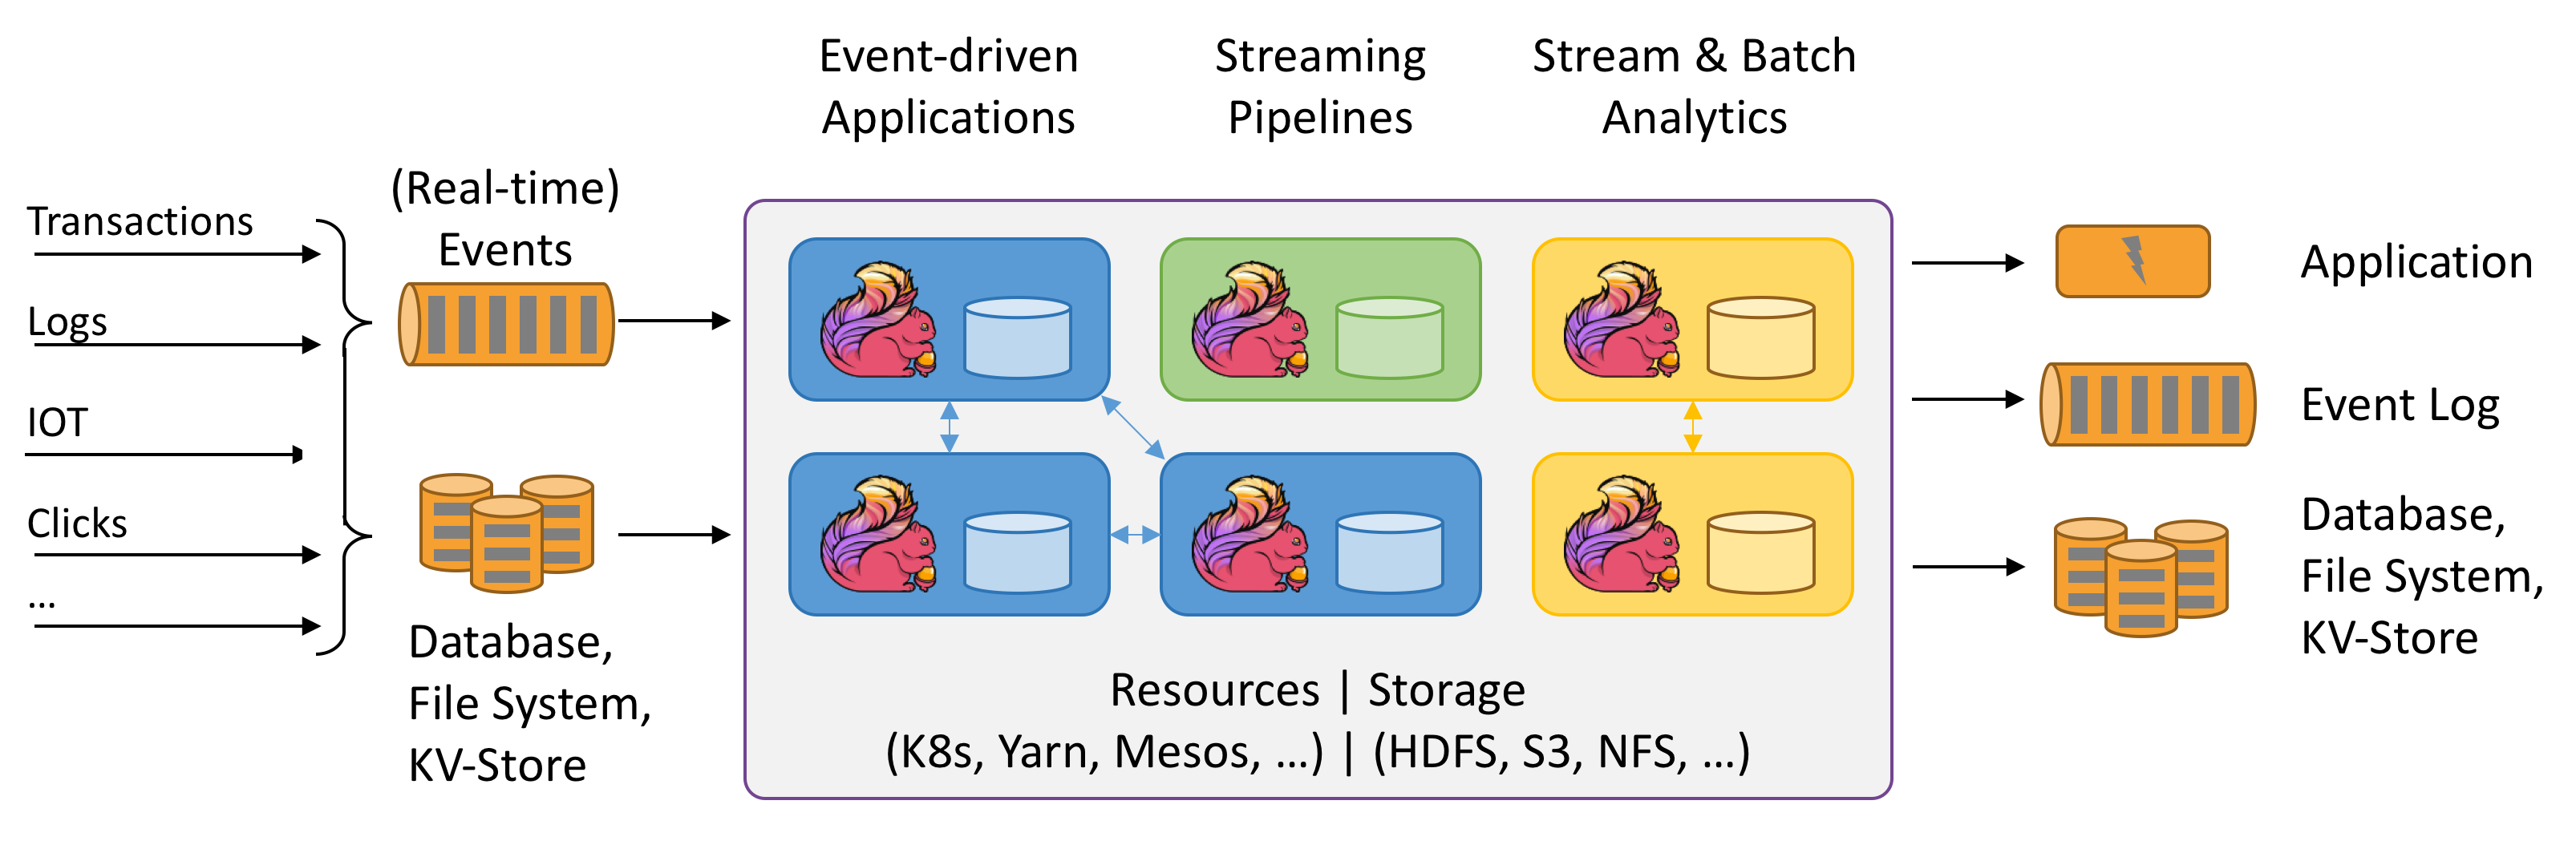
\includegraphics[width=\textwidth]{flink-home-graphic.png}

\textbf{Flink几大模块}

\begin{itemize}
\item Flink Table and SQL(还没开发完)
\item Flink Gelly(图计算)
\item Flink CEP(复杂事件处理)
\end{itemize}

\subsection{为什么选择Flink}

许多系统都会产生连续的事件流,如行驶中的汽车发射出GPS信号,金融交易,移动通信基站与繁忙的智能手机进行信号交换,网络流量,机器日志,工业传感器和可穿戴设备的测量结果,等等。如果能够高效地分析大规模流数据,我们对上述系统的理解将会更清楚、更快速。简而言之,流数据更真实地反映了我们的生活方式。

实际上,企业常见的数据架构仍旧假设数据是有头有尾的有限集。这个假设存在的大部分原因在于,与有限集匹配的数据存储及处理系统建起来比较简单。但是,这样做无疑给那些天然的流式场景人为地加了限制。

我们渴望按照流的方式处理数据,但要做好很困难; 随着大规模数据在各行各业中出现,难度越来越大。这是一个属于物理学范畴的难题: 在大型分布式系统中,数据一致性和对事件发生顺序的理解必然都是有限的。

而Flink为大容量数据提供流处理,并用同一种技术实现批处理。

\subsubsection{流处理欠佳的后果}

谁需要和流数据打交道呢? 首先映入脑海的是从事传感器测量和金融交易的工作人员。对于他们来说,流处理非常有用。但是流数据来源非常广泛,两个常见的例子是: 网站获得的能够反映用户行为的点击流数据,以及私有数据中心的机器日志。事实上,流数据来源无处不在,但是从连续事件中获得数据并不意味着可以在批量计算中使用这些数据。如今,处理大规模流数据的新技术正在改变这一状况。

\paragraph{零售业和市场营销}

在现代零售业中,网站点击量就代表了销量。网站获得的点击数据可能是大量、连续、不均匀的。用以往的技术很难处理好如此规模的数据。仅是构建批量系统处理这些数据流就很有挑战性: 结果很可能是需要一个庞大且复杂的系统。并且,传统的做法还会带来数据丢失、延迟、错误的聚合结果等问题。这样的结果怎能对商业领域有所帮助呢?

假设你正在向首席执行官汇报上一季度的销售数据,你肯定不想事后因为使用了不准确的数据而不得不向首席执行官更正汇报结果。如果不能良好地处理点击数据,你很可能对网站点击量进行不准确的计算,这将导致广告投放报价和业绩数字不准确。

航空旅客服务业面临同样的挑战: 航空公司需要快速、准确地处理从各种渠道获得的大量数据。例如,当为一名旅客办理登机手续时,需要对该旅客的机票预订数据进行核对,还需要核对行李处理信息、航班状态信息和账单信息。如果没有强大的技术来支持流处理,这种规模的数据是很难不出错的。近几年,美国四大航空公司中有三家都出现了大面积的服务中断,这几次故障都可以归咎于大规模实时数据处理失败。

当然,很多相关问题(如怎样避免重复预订酒店或演唱会门票),一般都能够通过有效的数据库操作来解决,但是这种操作相当费钱,也费精力。尤其当数据量增加时,成本会飙升,并且在某些情况下,数据库的反应速度会变得特别慢。由于缺乏灵活性,开发速度受到影响,项目在庞大又复杂或者不断发生变化的系统中进展缓慢。想要在大型系统中处理流数据,并且在保持一致性的同时有效地控制成本,难度非常大。

幸运的是,现代的流处理器经常可以用新的方式解决这些问题,这使得实时处理大规模数据的成本更低。流处理还激发了新的尝试,比如构建一个系统,该系统能够基于顾客当下购买的商品实时给出相关的建议,看看他们是否还需要买一些别的商品。这不代表流处理器替代了数据库(远远不能替代),而是说在数据库处理不好时,流处理器提供了更好的解决方案。这样做也使数据库得以解脱,不用再参与对当前业务状态的实时分析。

\paragraph{物联网}

物联网是流数据被普遍应用的领域。在物联网中,低延迟的数据传输和处理,以及准确的数据分析通常很关键。各类仪器中的传感器频繁地获得测量数据,并将它们以流的形式传输至数据中心。在数据中心内,实时或者接近实时的应用程序将更新显示板,运行机器学习模型,发布警告,并就许多不同的服务项目提供反馈。

交通运输业也体现了流处理的重要性。举例来说,先进的列车系统依靠的是传感器测量数据,这些数据从轨道传至列车,再从列车传至沿途的传感器; 与此同时,报告也被发送回控制中心。测量数据包括列车的速度和位置,以及轨道周边的状况。如果流数据没有被正确处理,调整意见和警告就不能相应产生,从而也就不能通过对危险状况做出反应来避免事故发生。

另一个例子是"智能"汽车,或称联网汽车,它们通过移动网络将数据传输回制造商。在有些国家(北欧国家、法国和英国,美国则刚开始),联网汽车甚至可以将信息传给保险公司; 如果是赛车,信息还可以通过射频链路传送至维修站进行分析。此外,一些智能手机应用程序还支持数百万司机共享实时路况信息。

物联网对公用事业也有影响。相关公司已经开始安装智能计量表,以替换每个月需要人工读数的旧表。智能计量表可以定期将用电量反馈给公司(例如每15分钟一次)。有些公司正在尝试每30秒就进行一次测量。使用智能计量表的这一转变带来了大量的流数据,同时也获得了大量的潜在收益。其中一个好处就是通过机器学习模型来检测设备故障或者窃电等使用异常。如果不能对流数据进行高吞吐、低延迟和准确的处理,这些新的目标都无法实现。

如果流处理做得不好,其他物联网项目也会遭殃。大型设备,比如风力涡轮机、生产设备和钻井泵,都依赖对传感器测量数据的分析来获得故障警告。如果不能及时地处理好这些设备的流数据,将可能付出高昂的代价,甚至导致灾难性后果。

\paragraph{电信业}

电信业是一个特殊的例子,它广泛地应用了基于各种目的而产生的跨地域的事件流数据。如果电信公司不能很好地处理流数据,就不能在某个移动通信基站出现流量高峰前预先将流量分配给其他的基站,也不能在断电时快速做出反应。通过处理流数据来进行异常检测,如检测通话中断或者设备故障,对于电信业来说至关重要。

\paragraph{银行和金融业}

因为流处理做得不好而给银行以及金融业带来的潜在问题是极其显著的。从事零售业务的银行不希望客户交易被延迟或者因为错误统计而造成账户余额出错。曾有一个说法叫作"银行家工作时间",指的就是银行需要在下午早早关门进行结算,这样才能保证第二天营业之前算出准确的账。这种批量作业的营业模式早已消失。如今,交易和报表都必须快速且准确地生成; 有些新兴的银行甚至提供实时的推送通知,以及随时随地访问手机银行的服务。在全球化经济中,能够提供24小时服务变得越来越重要。

那么,如果缺少能够灵敏地实时检测出用户行为异常的应用程序,会对金融机构带来什么后果呢? 信用卡欺诈检测需要及时的监控和反馈。对异常登录的检测能发现钓鱼式攻击,从而避免巨大的损失。

\subsubsection{连续事件处理的目标}

能够以非常低的延迟处理数据,这并不是流处理的唯一优势。人们希望流处理不仅做到低延迟和高吞吐,还可以处理中断。优秀的流处理技术应该能使系统在崩溃之后重新启动,并且产出准确的结果; 换句话说,优秀的流处理技术可以容错,而且能保证exactly-once。

与此同时,获得这种程度的容错性所采用的技术还需要在没有数据错误的情况下不产生太大的开销。这种技术需要能够基于事件发生的时间(而不是随意地设置处理间隔)来保证按照正确的顺序跟踪事件。对于开发人员而言,不论是写代码还是修正错误,系统都要容易操作和维护。同样重要的是,系统生成的结果需要与事件实际发生的顺序一致,比如能够处理乱序事件流(一个很不幸但无法避免的事实),以及能够准确地替换流数据(在审计或者调试时很有用)。

\subsubsection{流处理技术的演变}

分开处理连续的实时数据和有限批次的数据,可以使系统构建工作变得更加简单,但是这种做法将管理两套系统的复杂性留给了系统用户: 应用程序的开发团队和DevOps团队需要自己使用并管理这两套系统。

为了处理这种情况,有些用户开发出了自己的流处理系统。在开源世界里,Apache Storm项目(以下简称Storm)是流处理先锋。Storm提供了低延迟的流处理,但是它为实时性付出了一些代价: 很难实现高吞吐,并且其正确性没能达到通常所需的水平。换句话说,它并不能保证exactly-once; 即便是它能够保证的正确性级别,其开销也相当大。

\begin{bclogo}[logo=\bcinfo, couleurBarre=orange, noborder=true, couleur=white]{笔记}
若要依靠多个流事件来计算结果,必须将数据从一个事件保留到下一个事件。这些保存下来的数据叫作计算的状态。准确处理状态对于计算结果的一致性至关重要。在故障或中断之后能够继续准确地更新状态是容错的关键。
\end{bclogo}

在低延迟和高吞吐的流处理系统中维持良好的容错性是非常困难的,但是为了得到有保障的准确状态,人们想出了一种替代方法: 将连续事件中的流数据分割成一系列微小的批量作业。如果分割得足够小(即所谓的微批处理作业),计算就几乎可以实现真正的流处理。因为存在延迟,所以不可能做到完全实时,但是每个简单的应用程序都可以实现仅有几秒甚至几亚秒的延迟。这就是在Spark批处理引擎上运行的Apache Spark Streaming所使用的方法。

更重要的是,使用微批处理方法,可以实现exactly-once语义,从而保障状态的一致性。如果一个微批处理作业失败了,它可以重新运行。这比连续的流处理方法更容易。Storm Trident是对Storm的延伸,它的底层流处理引擎就是基于微批处理方法来进行计算的,从而实现了exactly-once语义,但是在延迟性方面付出了很大的代价。

然而,通过间歇性的批处理作业来模拟流处理,会导致开发和运维相互交错。完成间歇性的批处理作业所需的时间和数据到达的时间紧密耦合,任何延迟都可能导致不一致(或者说错误)的结果。这种技术的潜在问题是,时间由系统中生成小批量作业的那一部分全权控制。Spark Streaming等一些流处理框架在一定程度上弱化了这一弊端,但还是不能完全避免。另外,使用这种方法的计算有着糟糕的用户体验,尤其是那些对延迟比较敏感的作业,而且人们需要在写业务代码时花费大量精力来提升性能。

为了实现理想的功能,人们继续改进已有的处理器(比如Storm Trident的开发初衷就是试图克服Storm的局限性)。当已有的处理器不能满足需求时,产生的各种后果则必须由应用程序开发人员面对和解决。以微批处理方法为例,人们往往期望根据实际情况分割事件数据,而处理器只能根据批量作业时间(恢复间隔)的倍数进行分割。当灵活性和表现力都缺乏的时候,开发速度变慢,运维成本变高。

于是,Flink出现了。这一数据处理器可以避免上述弊端,并且拥有所需的诸多功能,还能按照连续事件高效地处理数据。Flink 的一些功能如下图所示。

与Storm和Spark Streaming类似,其他流处理技术同样可以提供一些有用的功能,但是没有一个像Flink那样功能如此齐全。举例来说,Apache Samza(以下简称Samza)是早期的一个开源流处理器,它不仅没能实现exactly-once语义,而且只能提供底层的API; 同样,Apache Apex提供了与Flink相同的一些功能,但不全面(比如只提供底层的API,不支持事件时间,也不支持批量计算)。这些项目没有一个能和Flink在开源社区的规模上相提并论。

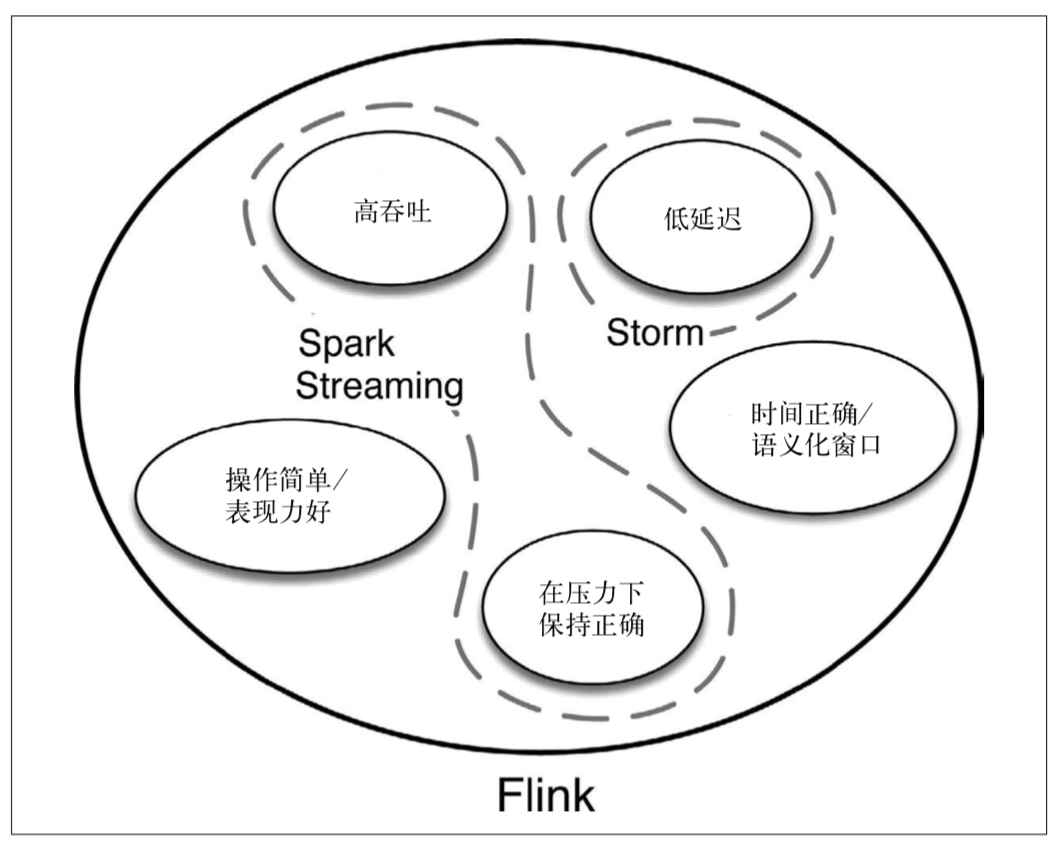
\includegraphics[width=\textwidth]{flinkvsother.png}

Flink的一个优势是,它拥有诸多重要的流式计算功能。其他项目为了实现这些功能,都不得不付出代价。比如,Storm实现了低延迟,但是做不到高吞吐,也不能在故障发生时准确地处理计算状态; Spark Streaming通过采用微批处理方法实现了高吞吐和容错性,但是牺牲了低延迟和实时处理能力,也不能使窗口与自然时间相匹配,并且表现力欠佳。

*Spark Streaming* vs *Flink*

1. 两者最重要的区别(流和微批)

(1). Micro Batching 模式(spark)

Micro-Batching计算模式认为"流是批的特例",流计算就是将连续不断的批进行持续计算,如果批足够小那么就有足够小的延时,在一定程度上满足了99%的实时计算场景。那么那1%为啥做不到呢? 这就是架构的魅力,在Micro-Batching模式的架构实现上就有一个自然流数据流入系统进行攒批的过程,这在一定程度上就增加了延时。具体如下示意图:

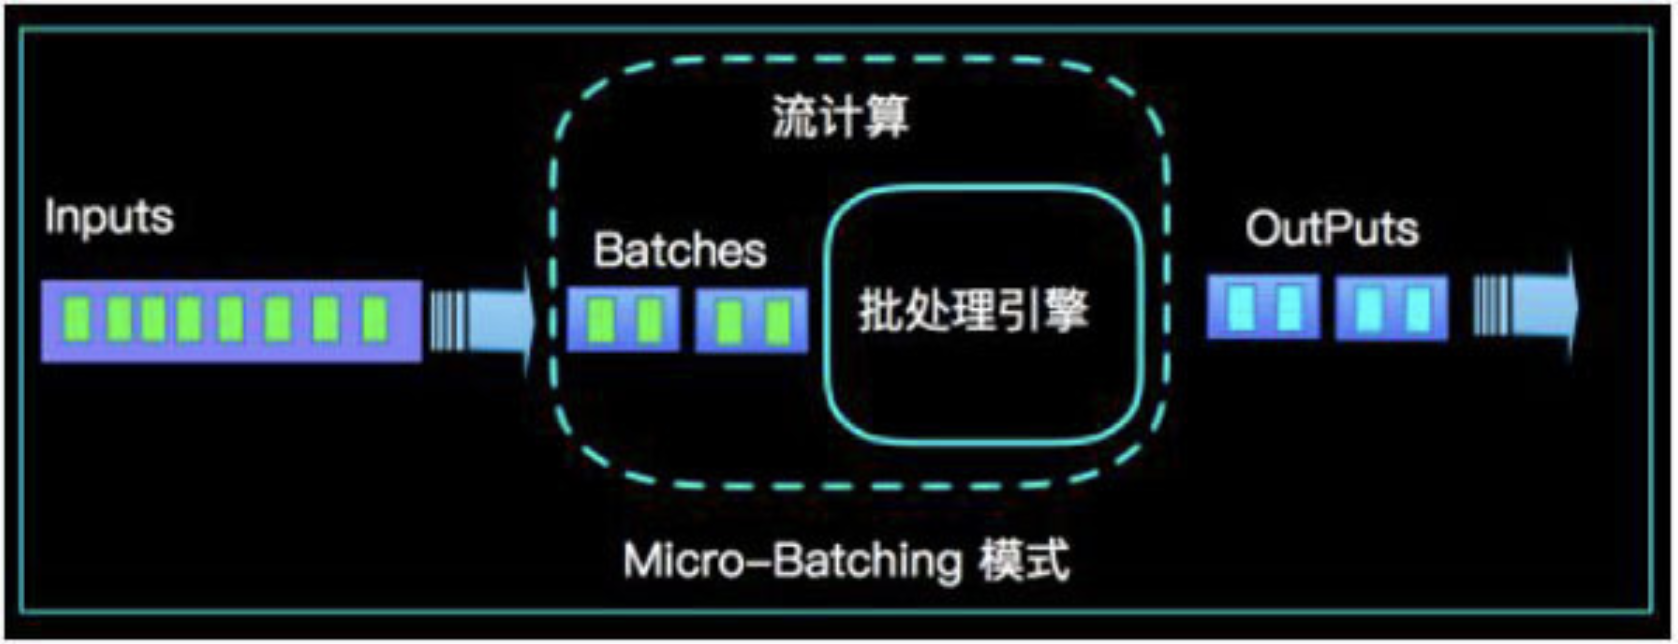
\includegraphics[width=\linewidth]{sparkstreamingvsflink1.png}

从上面可以看到是把输入的数据, 分成微小的批次, 然后一个批次一个批次的处理, 然后也是一片批次的输出. 很显然Micro-Batching模式有其天生的低延时瓶颈,但任何事物的存在都有两面性,在大数据计算的发展历史上,最初Hadoop上的MapReduce就是优秀的批模式计算框架,Micro-Batching在设计和实现上可以借鉴很多成熟实践。

(2). Native Streaming 模式(flink)

Native Streaming计算模式认为批是流的特例",这个认知更贴切流的概念,比如一些监控类的消息流,数据库操作的binlog,实时的支付交易信息等等自然流数据都是一条,一条的流入。Native Streaming计算模式每条数据的到来都进行计算,这种计算模式显得更自然,并且延时性能达到更低。具体如下示意图:

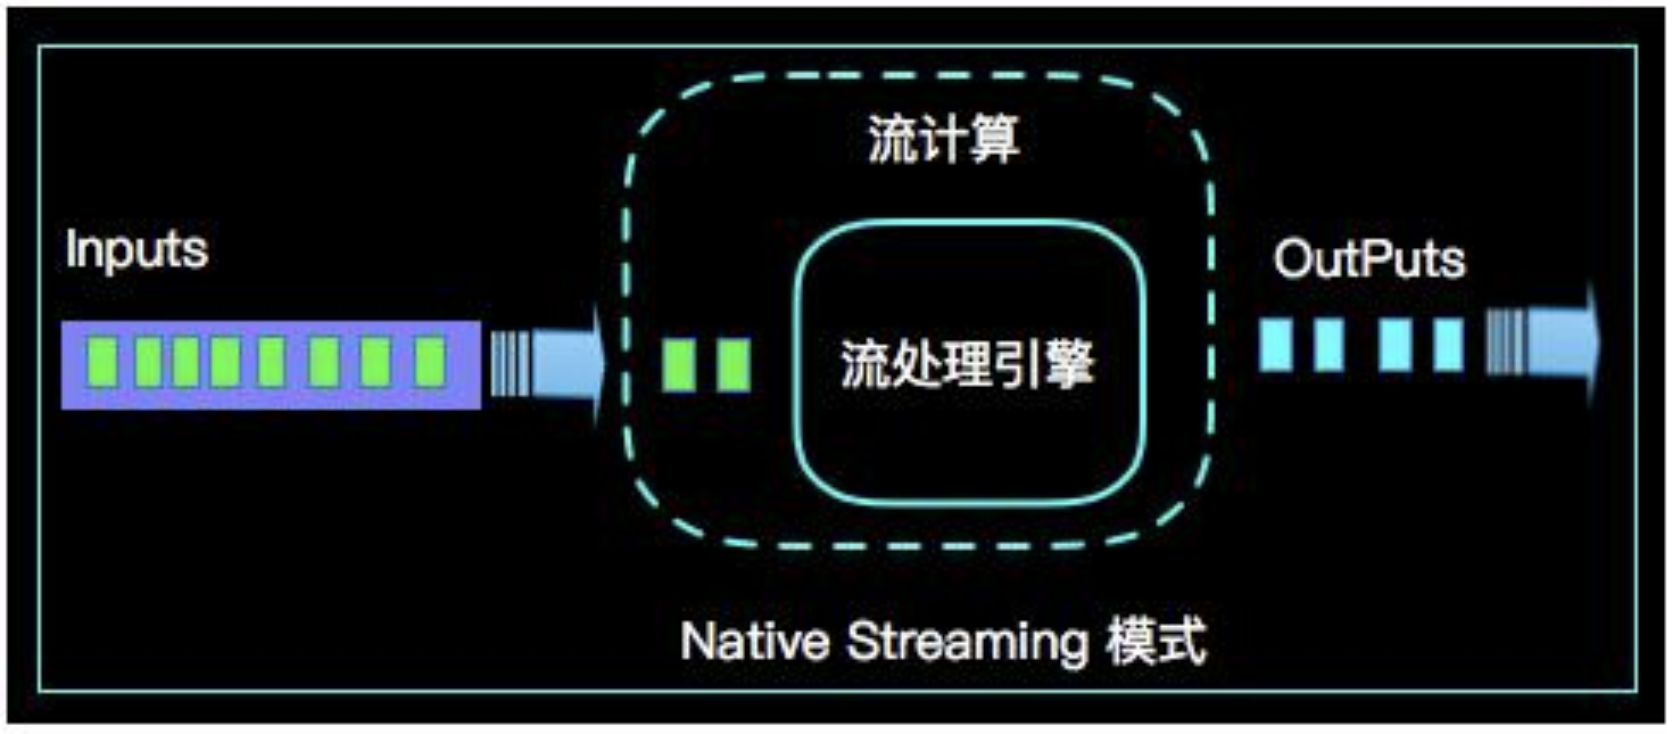
\includegraphics[width=\textwidth]{sparkstreamingvsflink2.png}

从上图可以看到输入的数据过来一条处理一条, 然后输出, 几乎不存在延迟, 很明显Native Streaming模式占据了流计算领域"低延时"的核心竞争力, 当然Native Streaming模式的实现框架是一个历史先河,第一个实现Native Streaming模式的流计算框架是第一个吃螃蟹的人,需要面临更多的挑战,后续章节我们会慢慢介绍。当然Native Streaming模式的框架实现上面很容易实现Micro-Batching和Batching模式的计算,Apache Flink就是Native Streaming计算模式的流批统一的计算引擎。

2. 数据模型

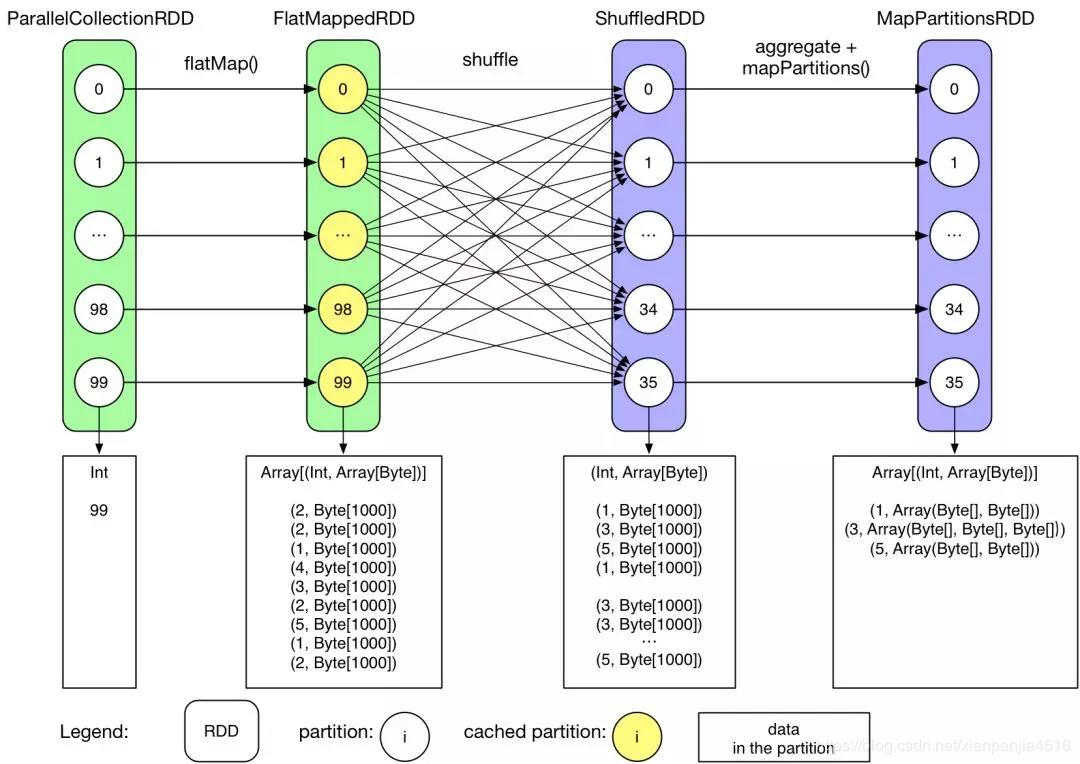
\includegraphics[width=\textwidth]{shujumoxing1.png}

Spark最早采用RDD模型,达到比MapReduce计算快100倍的显著优势,对Hadoop生态大幅升级换代。RDD弹性数据集是分割为固定大小的批数据,RDD提供了丰富的底层API对数据集做操作。为持续降低使用门槛,Spark社区开始开发高阶API:DataFrame/DataSet,Spark SQL作为统一的API,掩盖了底层,同时针对性地做SQL逻辑优化和物理优化,非堆存储优化也大幅提升了性能。

Spark Streaming里的DStream和RDD模型类似,把一个实时进来的无限数据分割为一个个小批数据集合DStream,定时器定时通知处理系统去处理这些微批数据。劣势非常明显,API少、难胜任复杂的流计算业务,调大吞吐量而不触发背压是个体力活。不支持乱序处理,或者说很难处理乱序的问题。Spark Streaming仅适合简单的流处理,这里稍微解释一下,因为Spark的创始人在当时认为延迟不是那么的重要,他认为现实生活中没有那么多低延迟的应用场景,所以就没太注重延迟的问题,但是随着生活多样化场景的不断增加,对实时性的要求越来越高,所以Spark也注意到了这个问题,开始在延迟方面发力,进而推出了Structured Streaming,相信很快Spark Streaming就会被Structured Streaming替代掉。

Spark Structured Streaming提供了微批和流式两个处理引擎。微批的API虽不如Flink丰富,窗口、消息时间、trigger、watermarker、流表join、流流join这些常用的能力都具备了。时延仍然保持最小100毫秒。当前处在试验阶段的流式引擎,提供了1毫秒的时延,但不能保证exactly-once语义,支持at-least-once语义。同时,微批作业打了快照,作业改为流式模式重启作业是不兼容的。这一点不如Flink做的完美。当然了现在还在优化阶段.

综上,Spark Streaming和Structured Streaming是用批计算的思路做流计算。其实,用流计算的思路开发批计算才是最合理的。对Spark来讲,大换血不大可能,只有局部优化。其实,Spark里core、streaming、structured streaming、graphx四个模块,是四种实现思路,通过上层SQL统一显得不纯粹和谐。

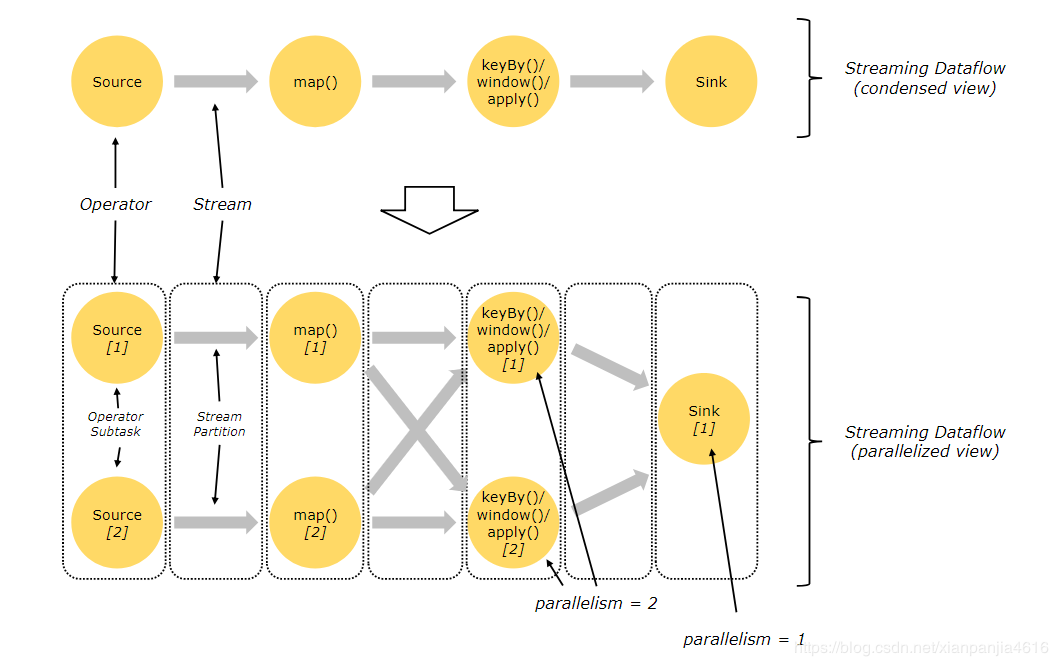
\includegraphics[width=\textwidth]{shujumoxing2.png}

Flink的基本数据模型是数据流,及事件(Event)的序列。数据流作为数据的基本模型可能没有表或者数据块直观熟悉,但是可以证明是完全等效的。流可以是无边界的无限流,即一般意义上的流处理。也可以是有边界的有限流,这样就是批处理。

Flink采用Dataflow模型,和Lambda模式不同。Dataflow是纯粹的节点组成的一个图,图中的节点可以执行批计算,也可以是流计算,也可以是机器学习算法,流数据在节点之间流动,被节点上的处理函数实时apply处理,节点之间是用netty连接起来,两个netty之间keepalive,网络buffer是自然反压的关键。经过逻辑优化和物理优化,Dataflow的逻辑关系和运行时的物理拓扑相差不大。这是纯粹的流式设计,时延和吞吐理论上是最优的。

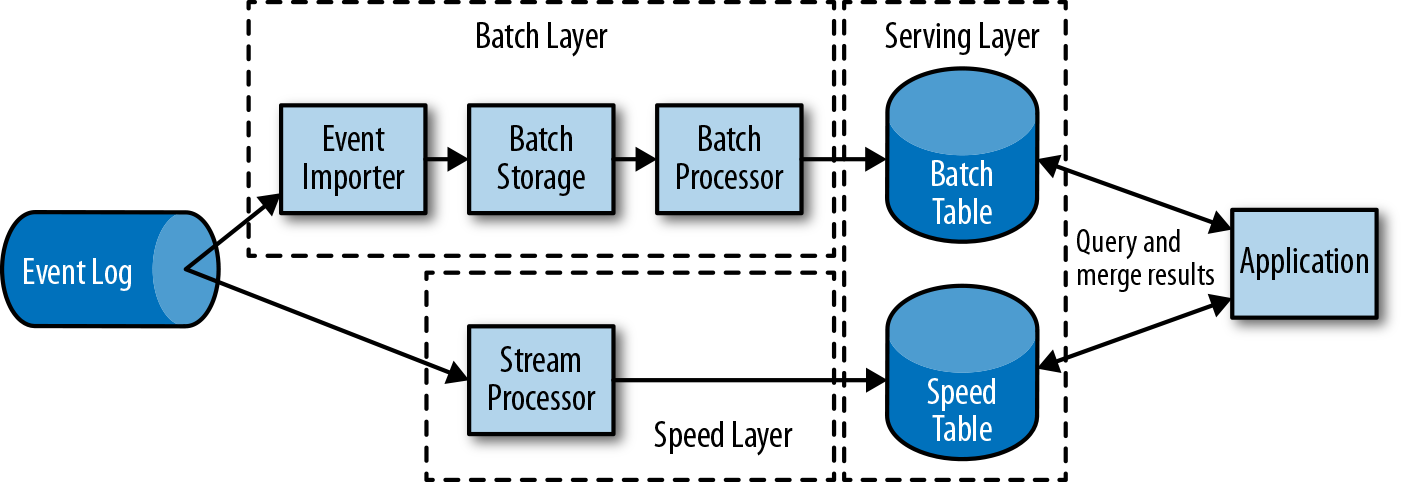
\includegraphics[width=\textwidth]{lambdaarch.png}

3. 运行时架构

*Spark运行时架构*

批计算是把DAG划分为不同stage,DAG节点之间有血缘关系,在运行期间一个stage的task任务列表执行完毕,销毁再去执行下一个stage;Spark Streaming则是对持续流入的数据划分一个批次,定时去执行批次的数据运算。Structured Streaming将无限输入流保存在状态存储中,对流数据做微批或实时的计算,跟Dataflow模型比较像。

*Flink运行时架构*

Flink有统一的runtime,在此之上可以是Batch API、Stream API、ML、Graph、CEP等,DAG中的节点上执行上述模块的功能函数,DAG会一步步转化成ExecutionGraph,即物理可执行的图,最终交给调度系统。节点中的逻辑在资源池中的task上被apply执行,task和Spark中的task类似,都对应线程池中的一个线程。

在DAG的执行上,Spark和Flink有一个比较显著的区别。在Flink的流执行模式中,一个事件在一个节点处理完后的输出就可以发到下一个节点立即处理。这样执行引擎并不会引入额外的延迟。与之相应的,所有节点是需要同时运行的。而Spark的micro batch和一般的batch执行一样,处理完上游的stage得到输出之后才开始下游的stage。

在流计算的运行时架构方面,Flink明显更为统一且优雅一些。

\begin{bclogo}[logo=\bcinfo, couleurBarre=orange, noborder=true, couleur=white]{笔记}
Lambda架构的问题是改变代码后需要重新在两个复杂的分布式系统中再次处理输出结果是非常痛苦的,而且我不认为这个问题能够解决。相当于同一套数据集的处理逻辑,使用Spark Core需要写一遍,使用Spark Streaming需要再写一遍,无法复用,这是致命缺陷。
\end{bclogo}

\subsection{Flink的重要特点}

\subsubsection{事件驱动型(Event-Driven)}

事件驱动型应用是一类具有状态的应用,它从一个或多个事件流提取数据,并根据到来的事件触发计算、状态更新或其他外部动作。比较典型的就是以Kafka为代表的消息队列几乎都是事件驱动型应用。

与之不同的就是Spark Streaming微批次,如图:

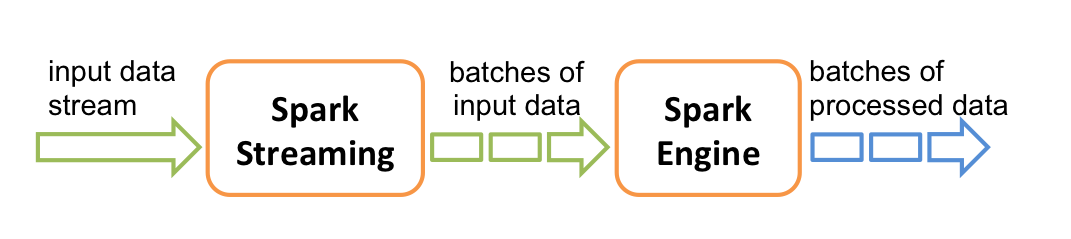
\includegraphics[width=\textwidth]{streaming-flow.png}

事件驱动型:

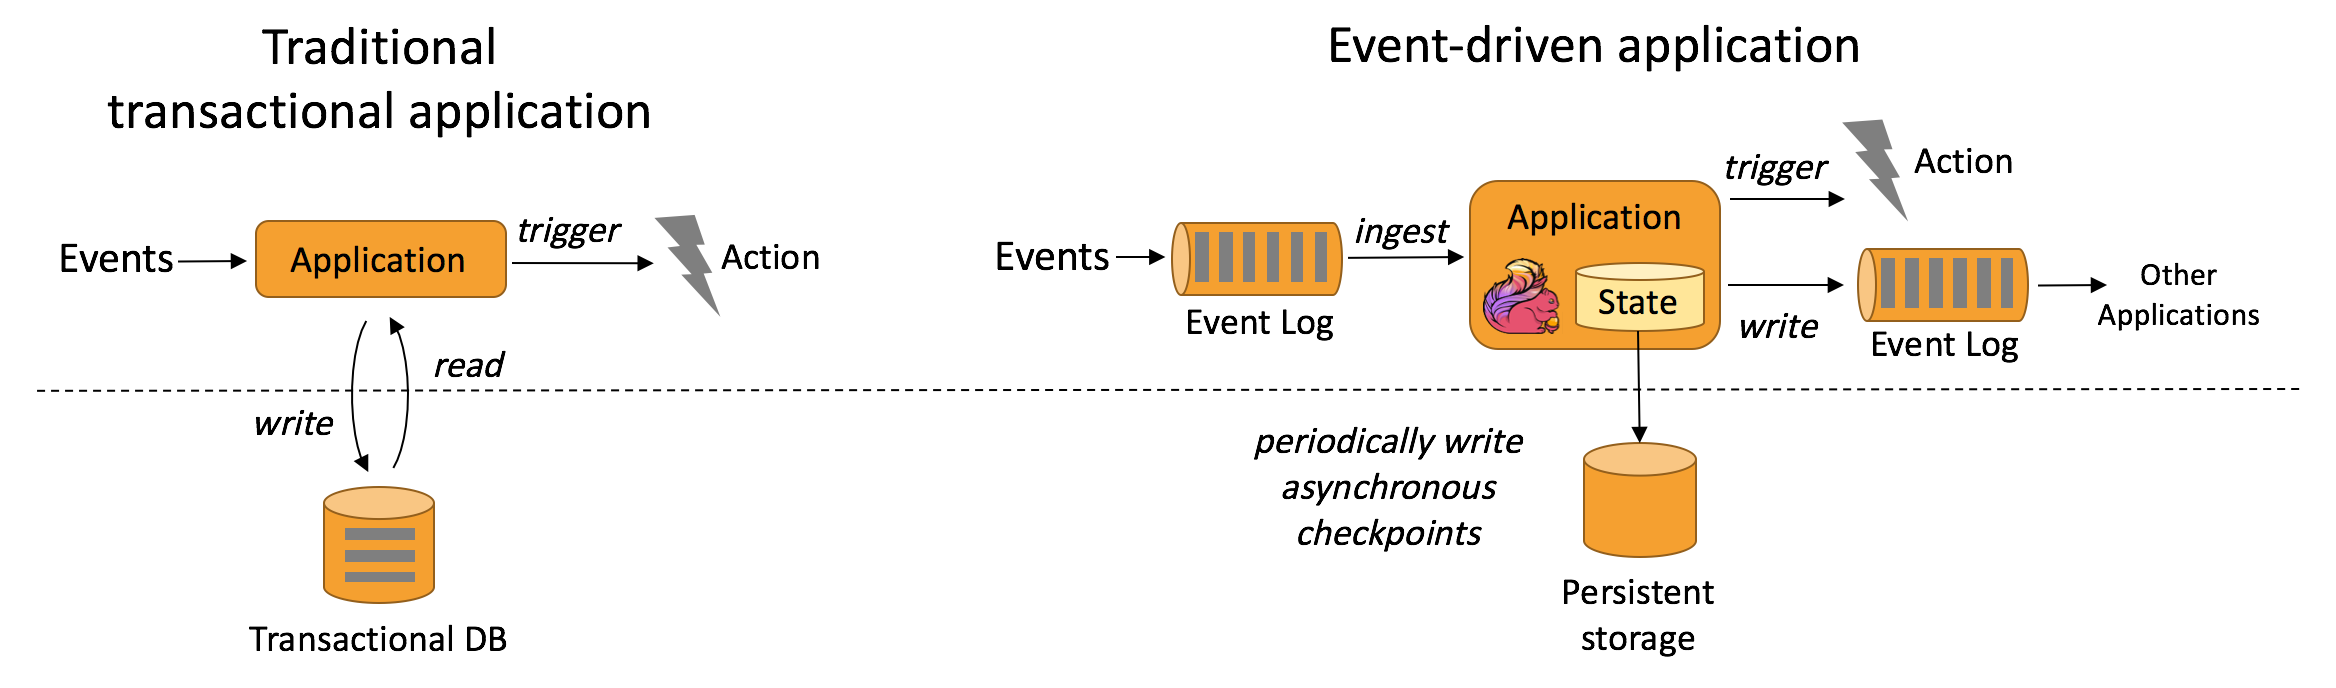
\includegraphics[width=\textwidth]{usecases-eventdrivenapps.png}

==== 1.3.2 流与批的世界观

**批处理**的特点是有界、持久、大量,非常适合需要访问全套记录才能完成的计算工作,一般用于离线统计。

**流处理**的特点是无界、实时,无需针对整个数据集执行操作,而是对通过系统传输的每个数据项执行操作,一般用于实时统计。

在Spark的世界观中,一切都是由批次组成的,离线数据是一个大批次,而实时数据是由一个一个无限的小批次组成的。

而在Flink的世界观中,一切都是由流组成的,离线数据是有界限的流,实时数据是一个没有界限的流,这就是所谓的有界流和无界流。

*无界数据流*:无界数据流有一个开始但是没有结束,它们不会在生成时终止并提供数据,必须连续处理无界流,也就是说必须在获取后立即处理event。对于无界数据流我们无法等待所有数据都到达,因为输入是无界的,并且在任何时间点都不会完成。处理无界数据通常要求以特定顺序(例如事件发生的顺序)获取event,以便能够推断结果完整性。

*有界数据流*:有界数据流有明确定义的开始和结束,可以在执行任何计算之前通过获取所有数据来处理有界流,处理有界流不需要有序获取,因为可以始终对有界数据集进行排序,有界流的处理也称为批处理。

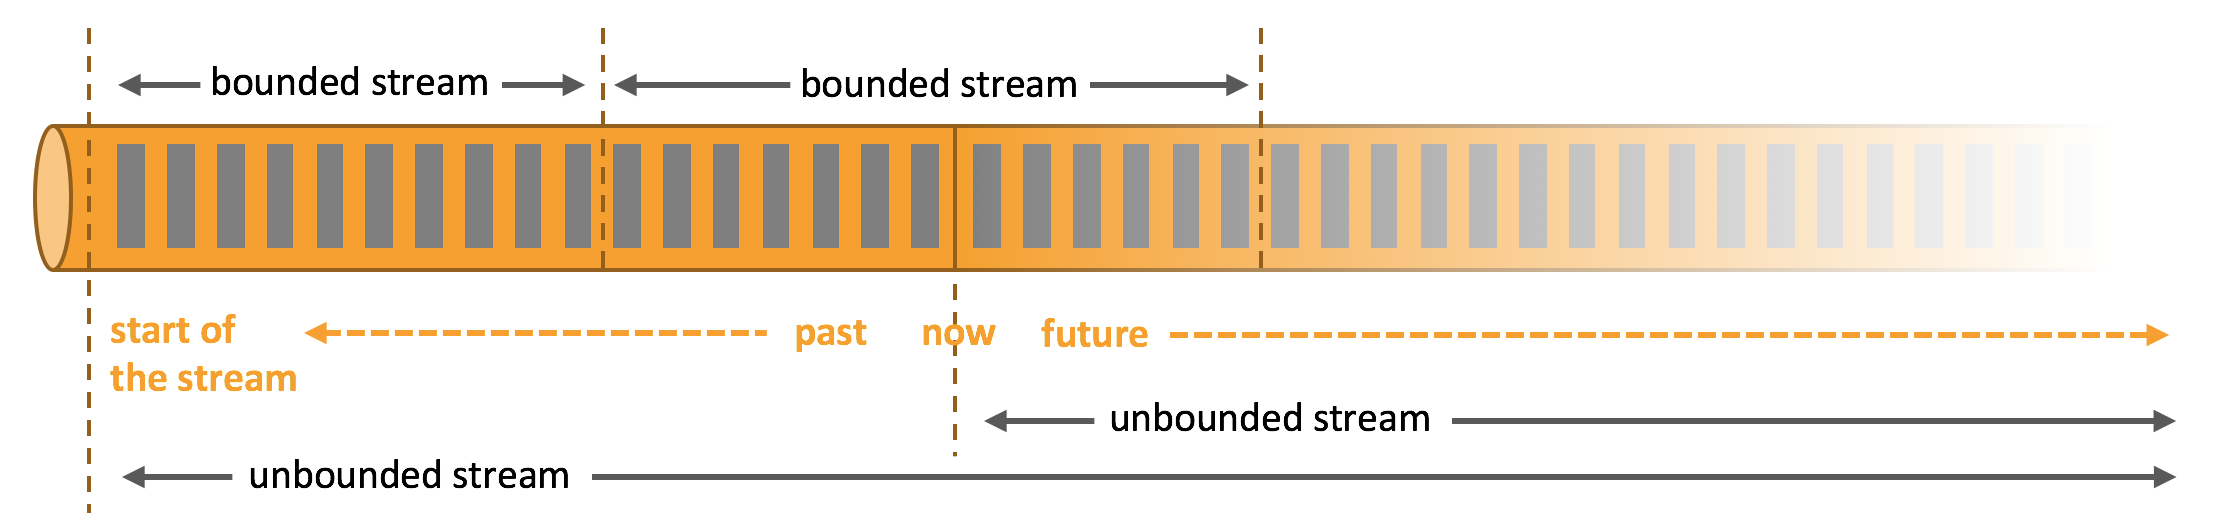
\includegraphics[width=\textwidth]{bounded-unbounded.png}

这种以流为世界观的架构,获得的最大好处就是具有极低的延迟。

\subsubsection{分层api}

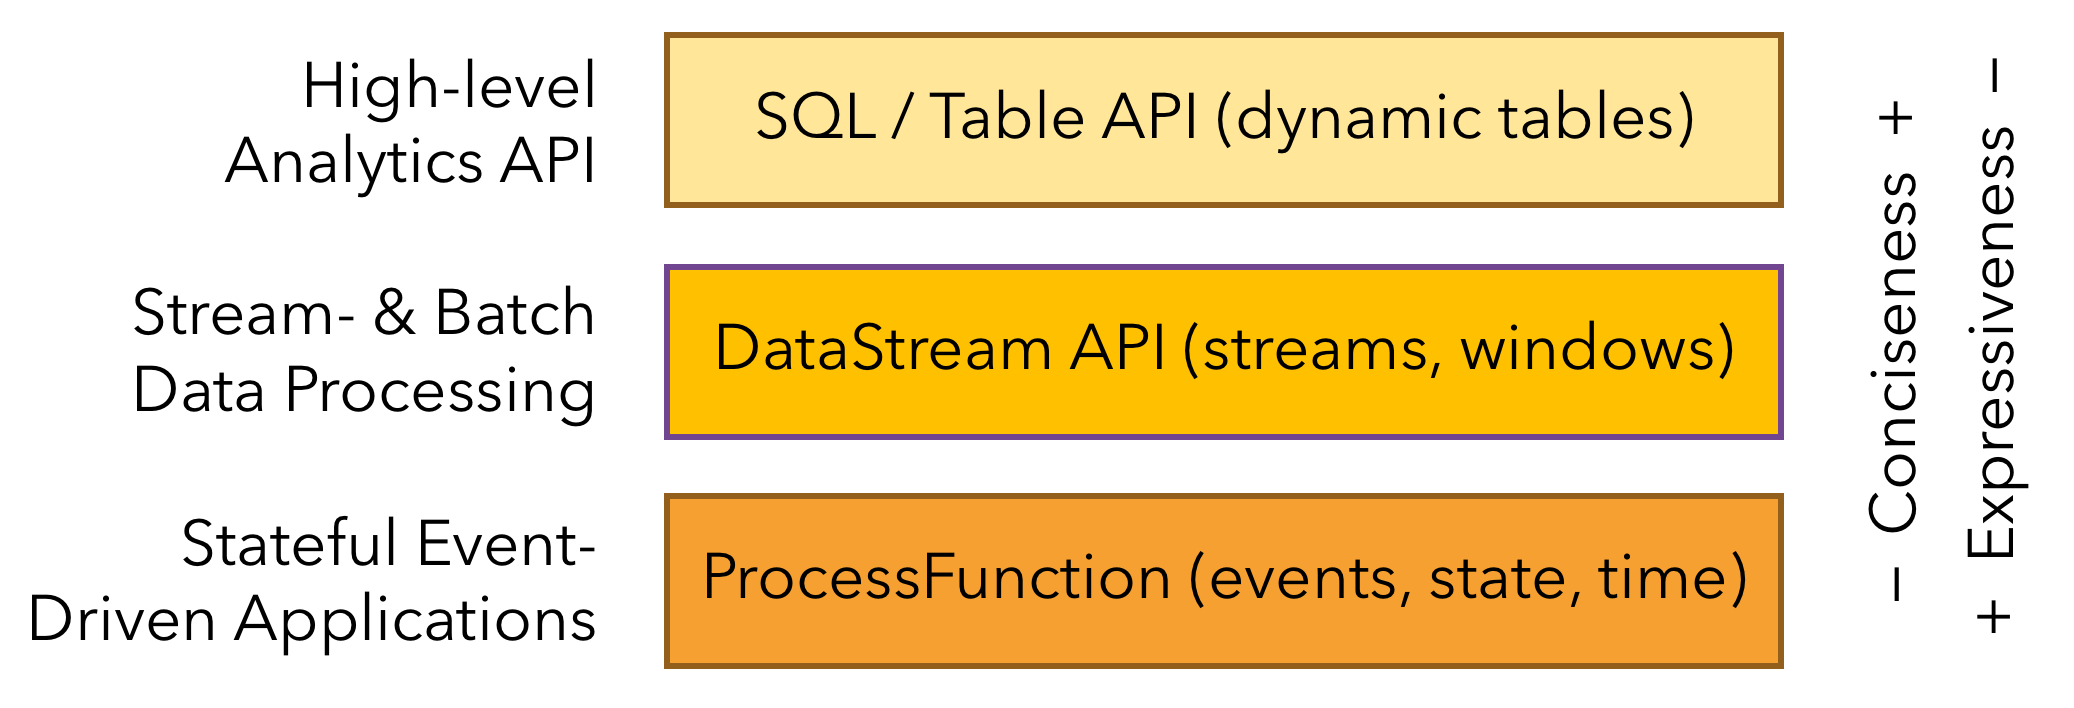
\includegraphics[width=\textwidth]{api-stack.png}

最底层级的抽象仅仅提供了有状态流,它将通过在DataStream API中嵌入Process Function来处理数据。Process Function与DataStream API相集成,使其可以对某些特定的操作进行底层的抽象,它允许用户可以自由地处理来自一个或多个数据流的事件,并使用一致的容错的状态。除此之外,用户可以注册事件时间并处理时间回调,从而使程序可以处理复杂的计算。

实际上,大多数应用并不需要上述的底层抽象,而是针对核心API(Core APIs)进行编程,比如DataStream API(有界或无界流数据)以及DataSet API(有界数据集)。这些API为数据处理提供了通用的构建模块,比如由用户定义的多种形式的转换(transformations),连接(joins),聚合(aggregations),窗口操作(window)等等。DataSet API为有界数据集提供了额外的支持,例如循环与迭代。这些API处理的数据类型以类(classes)的形式由各自的编程语言所表示。

Table API是以表为中心的声明式编程,其中表可能会动态变化(在表达流数据时)。Table API遵循(扩展的)关系模型:表有二维数据结构(schema)(类似于关系数据库中的表),同时API提供与RDBMS相似的操作,例如select、project、join、group-by、aggregate等。Table API程序声明式地定义了什么逻辑操作应该执行,而不是准确地确定这些操作代码看上去如何(过程式编程风格)。尽管Table API可以通过多种类型的用户自定义函数(UDF)进行扩展,其仍不如核心API更具表达能力,但是使用起来却更加简洁(代码量更少)。除此之外,Table API程序在执行之前会经过内置优化器进行优化。

你可以在表与DataStream/DataSet之间无缝切换,以允许程序将Table API与DataStream以及DataSet混合使用。

Flink提供的最高层级的抽象是SQL。这一层抽象在语法与表达能力上与Table API类似,但是是以SQL查询表达式的形式表现程序。SQL抽象与Table API交互密切,同时SQL查询可以直接在Table API定义的表上执行。

WARNING: 目前Flink作为批处理还不是主流,不如Spark成熟,所以DataSet使用的并不是很多。Flink Table API和Flink SQL也并不完善,大多都由各大厂商自己定制。所以我们主要学习DataStream API的使用。实际上Flink作为最接近Google DataFlow模型的实现,是流批统一的观点,所以基本上使用DataStream就可以了。


== 第二章 Flink快速上手

=== 2.1 使用Maven搭建工程

*IDE推荐使用Idea*

我们使用Flink官方提供的flink-quickstart-scala原型来创建我们的工程,因为Flink官方提供的pom.xml经过了精心配置,可以打包出很小的Jar包。

image::quickstart1.png[]

image::quickstart2.png[]

image::quickstart3.png[]

image::quickstart4.png[]

image::quickstart5.png[]

image::quickstart6.png[]

image::quickstart7.png[]

[source,shell]
----
$ tree quickstart/
quickstart/
├── pom.xml
└── src
    └── main
        ├── resources
        │   └── log4j.properties
        └── scala
            └── org
                └── myorg
                    └── quickstart
                        ├── BatchJob.scala
                        └── StreamingJob.scala
----

.StreamingJob.scala
[source, scala]
----
package com.atguigu

import org.apache.flink.streaming.api.scala._ // 隐式类型转换
import org.apache.flink.streaming.api.windowing.time.Time

object StreamingJob {

  /** Main program method */
  def main(args: Array[String]) : Unit = {

    // get the execution environment
    val env: StreamExecutionEnvironment = StreamExecutionEnvironment.getExecutionEnvironment

    // get input data by connecting to the socket
    val text: DataStream[String] = env.socketTextStream("localhost", 9999, '\n')

    // parse the data, group it, window it, and aggregate the counts
    val windowCounts = text
      .flatMap { w => w.split("\\s") } // <1>
      .map { w => WordWithCount(w, 1) }
      .keyBy("word")
      .timeWindow(Time.seconds(5))
      .sum("count")

    // print the results with a single thread, rather than in parallel
    windowCounts.print().setParallelism(1)

    env.execute("Socket Window WordCount")
  }

  /** Data type for words with count */
  case class WordWithCount(word: String, count: Long)
}
----
<1> flatMap的函数签名:``def flatMap[A,B](as: List[A])(f: A => List[B]): List[B]``, 例如: ``flatMap(List(1,2,3))(i => List(i,i))``结果是``List(1,1,2,2,3,3)``, ``List("a b", "c d").flatMap(line => line.split(" "))``结果是``List(a, b, c, d)``。

新建一个Terminal终端,然后运行以下:

[source, shell]
----
$ nc -lk 9999
----

查看结果,在flink文件夹中的log文件夹里,后缀名为``.out``, 和在idea里面执行的样子不一样,不会打印到控制台。 

=== 2.2 Flink部署

==== 2.2.1 下载Hadoop Free版本的Flink

:download-link: https://www.apache.org/dyn/closer.lua/flink/flink-1.7.2/flink-1.7.2-bin-scala_2.11.tgz[下载链接]

{download-link}

==== 2.2.2 解压缩

[source,shell]
----
$ tar xvfz flink-1.7.2-bin-scala_2.11.tgz
----

==== 2.2.3 启动Flink集群

[source,shell]
----
$ cd flink-1.7.2
$ ./bin/start-cluster.sh
----

==== 2.2.4 在浏览器中打开Flink的Web UI

http://localhost:8081

==== 2.2.5 打包编写好的StreamingJob程序

在Idea中使用maven package功能打包。

==== 2.2.6 提交打包好的程序

[source,shell]
----
$ ./bin/flink run xxxx.jar
----

==== 2.2.7 在Flink Web UI查看Dashboard中job的执行状态

==== 2.2.8 停止Flink集群

[source,shell]
----
$ ./bin/stop-cluster.sh
----








\end{document}
